\chapter{Verfahren}
https://www.degruyter.com/document/doi/10.3139/104.112066/html
https://datasolut.com/was-ist-data-mining/
https://www.guru99.com/data-mining-tutorial.html

Die Verfahren des Data Mining können grob in zwei Teilgebiete unterteilt werden.

\begin{figure}[h!]
		\centering
		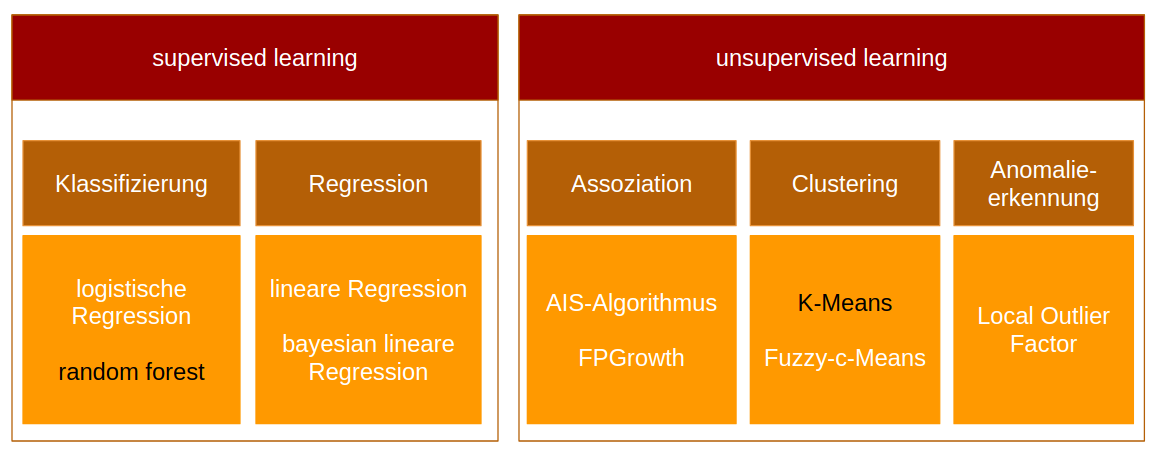
\includegraphics[width=1\textwidth]{verfahren.png}
		\caption{Übersicht der Verfahren (Quelle: Eigenkreation)}
\end{figure}

\section{Supervised Learning}
Beim supervised Learning (zu deutsch: überwachtes Lernen), sind die Zielwerte bekannt. Diese sind entweder aufgrund von Naturgestzen oder Expertenwissen gegeben. Ziel dieser Vorgehen ist es, einen Eingabewert einer dieser bekannten Zielwerte zuzuweisen.

\subsection{Klassifikationsverfahren}
\begin{figure}[h!]
	\centering
	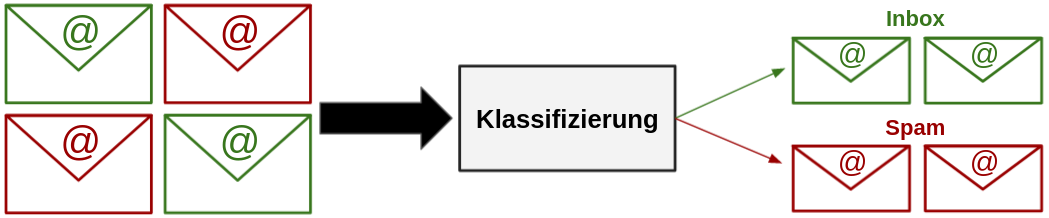
\includegraphics[width=1\textwidth]{classification.png}
	\caption{Klassifizierung von E-Mails (Quelle: Eigenkreation)}
\end{figure}
Bei der Klassifikation geht es darum, einen Datensatz einer Klasse aus einem gegeben Klassenpool zuzuweisen. Das einfachste Beispiel einer Klassifikation ist das erkennen von Spam-Mail. Hierbei haben wir den Klassenpool (Spam, nicht-Spam). Ein eigehendes Mail wird nun entweder der Klasse Spam oder der Klasse Nicht-Spam zugewiesen. Der Algorithmus, welcher diese Zuteilung macht, nennt sich Klassifikator.
Beim Mailbeispiel sprechen wir von einer binären Klassifikation, da wir genau zwei Klassen in unserem Klassenpool haben. Dem gegenüber steht die Multiklassenklassifizierung, bei der mehr als zwei Klassen im Klassenpool bestehen. Ein Beispiel hierzu ist die Klassifizierung von Früchten in die Klassen (Apfel, Birne, Orange, Aprikose).
Zu beachten gibt es hierbei, dass mit der Anzahl Klassen auch die Schwierigkeit der korrekten Klassifikation anwächst. Deshalb ist häufig eine binäre Klassifikation einer Multiklassenklassifizierung vorzuziehen, sofern sich das Problem entsprechend vereinfachen lässt.

Beispiele von Klassifikationsverfahren sind die logistische Regression oder Random Forest.

\subsection{Regressionsanalyse}
\begin{figure}[h!]
	\centering
	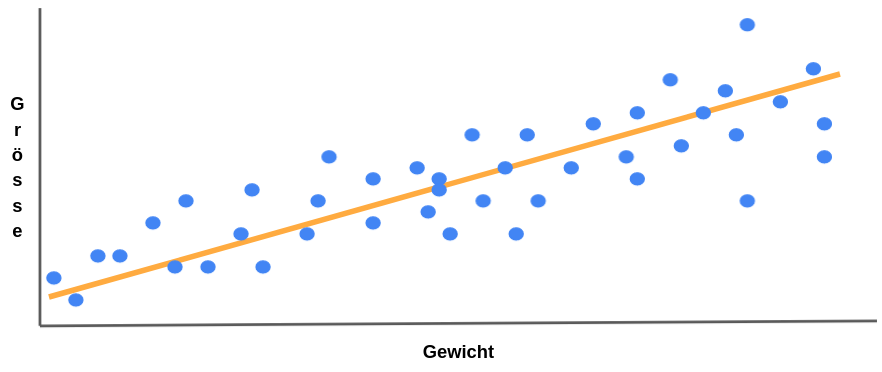
\includegraphics[width=1\textwidth]{regression.png}
	\caption{Bestimmung der Grösse durch Gewicht (Quelle: Eigenkreation)}
\end{figure}
Bei der Regressionsanlyse wird versucht, mittels einer abhängigen und einer oder mehreren unabhängigen Variablen ein Zusammenhang zu modellieren. Wichtig ist dabei die Abhängigkeit der ersten Variable. Fehlt diese funktioniert die Regression nicht. So ist es als Beispiel möglich, mittels Regression das Gewicht eines Menschen anhand seiner Körpergrösse zu modellieren, da grössere Menschen eher ein höheres Gewicht vorweisen. Jedoch ist es nicht möglich, aufgrund der Körpergrösse eines Menschen sein Jahreseinkommen vorauszusagen, da die beiden Variabeln unabhängig voneinander sind.
Eine einfache und häufige Art ist die lineare Regression. Hierbei wird versucht eine Funktion zu finden, die den Zusammenhang zwischen den variabeln möglichst genau beschreibt. Bei einer Einflüssgrösse (z. B. der Körpergrösse) und einer Zielgrösse (z. B. dem Gewicht), führt dies zu einer linearen Funktion.
Diese Funktion kann auf verschiedene Arten berechnet werden. Eine gängige Möglichkeit bildet hier die Methode der kleinsten quadratischen Abweichung. Dabei wird die lineare Funktion gesucht, welche zu allen gegebenen Datenpunkten die kleinst mögliche quadratische Abweichung erzielt.

Ein weiteres Beispiel für die Regression ist die bayesian lineare Regression.

\section{Unsupervised Learning}
Beim unsupervised learning (zu deutsch: unüberwachtes Lernen) sind im Gegensatz zum supervised learning die Zielwerte nicht bekannt. Bei diesen Verfahren wird versucht innerhalb der Daten Muster zu erkennen, damit neue Erkentnisse aus den Daten gezogen werden können.


\subsection{Assoziationsanalyse}
\begin{figure}[h!]
	\centering
	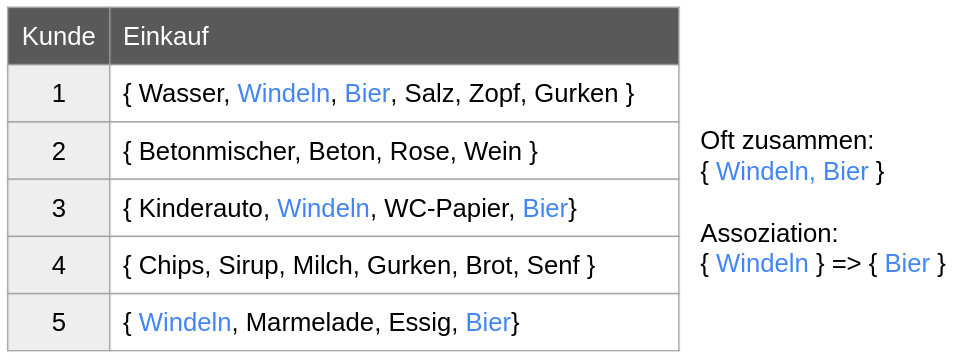
\includegraphics[width=1\textwidth]{association.png}
	\caption{Warenkorbanalyse (Quelle: Eigenkreation)}
\end{figure}
Bei der Assoziationsanalyse wird versucht eine Korrelation zwischen gemeinsam auftrettenden Items herzustellen.
Ein Item ist dabei ein Element einer gegebenen Menge. Durch Assoziation soll also herausgefunden werden, welche Items häufig gemeinsam auftretten. Ein häufiges Beispiel dazu ist die Analyse von Warenkörben. Dort wird versucht herauszufinden, welche Produkte häufig miteinander gekauft werden. So wurde als Beispiel herausgefunden, dass Männer zwischen 30 und 40 Jahre am Samstag häufig Windeln und Bier zusammen kaufen.

Zwei Beispiele für die Assoziationsanylse sind der AIS-Algorithmus und FPGrowth.

\subsection{Clusteranalyse}
\label{sec:clustering}
\begin{figure}[h!]
	\centering
	\includegraphics[width=1\textwidth]{clustering.png}
	\caption{Gruppieren durch Alter und Einkommen (Quelle: Eigenkreation)}
\end{figure}
Bei der CLusteranalyse geht es darum, Daten in verschiedene Gruppen einzuteilen. Das Ziel ist, dass jede Gruppe Elemente beinhaltet, die sich möglichst ähnlich sind. Inwiefer sich die Elemente ähnlich sind, spielt dabei für die Clusteranalyse keine Rolle. So kann die Ähnlichkeit bei Personendaten zum Beispiel aufgrund des Einkommens entstehen oder auch aufgrund der Herkunft der Personen. Auch eine Einteilung nach Alter wäre in so einem Falle denkbar. Wie die Ähnlichkeit bestimmt wird, hängt also davon ab, welche Daten (z. B. nur das Einkommen oder nur das Geschlecht) wir dem Algorithmus liefern.

Deshalb sind diese Gruppen am Anfang noch nicht zwangsläufig bekannt und werden erst durch die Analyse bestimmt. Sobald die Gruppen generiert wurden, kann untersucht werden welches die bestimmenden Merkmale einer Gruppe sind. Dies kann der Algorithmus nicht selber interpretieren. Die Interpretation der Gruppen ist ein seperater, oft manueller Schritt im Prozess. Hier sind allemvoran auch die Gruppen spannend, die wir nicht erwartet haben, da durch diese neue Informationen gewonnen werden. 

Oft verwendete Verfahren sind hierbei der K-Means-Algorithmus und der Fuzzy-c-Means-Algorithmus.

\subsection{Anomalieerkennung}
\begin{figure}[h!]
	\centering
	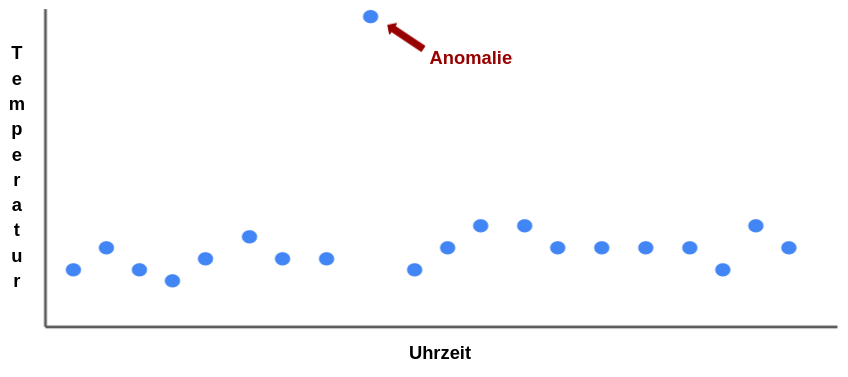
\includegraphics[width=1\textwidth]{anomanlie.png}
	\caption{Falsche Werte erkennen bei Wetterstation (Quelle: Eigenkreation)}
\end{figure}
Die Anomalieerkennung wird verwendet um zu erkennen, welche Datensätze nicht in ein bekanntes Muster passen. Es wird also konkret nach Ausreissern gesucht. Ein Beispiel hierzu sind Kreditkartendaten. Bei einer Kundin die normalerweise jeweils Beträge zwischen 50 und 200 Franken bezieht, wäre ein Bezug von mehreren Tausend Franken ein Ausreisser. Hierbei könnte es sich um eine betrügerische Aktion handeln. So könnte in diesem Beispiel durch den Ausreisser der Diebstahl der Karte festgestellt werden.
Ein weiteres Beispiel kann sein, Fehler in den Datenbeständen zu identifizieren. Eine Temperaturmessstation, die meist Werte zwischen 0 und 20 Grad liefert weisst wahrscheinlich eine Fehlfunktion auf, sollte sie einen Wert von 50 Grad liefern. Durch die Anomalieerkennung können solche Fehler ebenfalls schnell gefunden werden.

Ein bekannter Algorithums für diese Erkennung ist der Local Outlier Factor.

